
\documentclass[paper=a4,DIV15,oneside,lefteqn,american]{scrreprt}
\pdfoutput=1

\usepackage[american,german]{babel} 
\usepackage[margin=1.2in]{geometry}

\usepackage[T1]{fontenc}
\usepackage[utf8]{inputenc}

\usepackage{hyperref}
\usepackage[pdftex]{graphicx}
\usepackage{xspace}
\usepackage{textcomp}
\usepackage{framed}

\usepackage[draft,inline,nomargin]{fixme}

\usepackage{verbatim}

\usepackage{amsmath}
\usepackage{amssymb}
\usepackage{amsthm}
\usepackage{txfonts}
\usepackage{mathtools}

\addtolength{\parskip}{0.5\baselineskip}
\parindent=0cm



\newcommand{\VV}{Verification \& Validation\xspace}
\newcommand{\vv}{verification \& validation\xspace}

\def\CC{{C\nolinebreak[4]\hspace{-.05em}\raisebox{.4ex}{\tiny\bf ++}}}

\newcommand{\bitwalker}{\mbox{\texttt{Bitwalker}}\xspace}

\newcommand{\poke}{\mbox{\texttt{Bitwalker\_Poke}}\xspace}
\newcommand{\peek}{\mbox{\texttt{Bitwalker\_Peek}}\xspace}
\newcommand{\acsl}{\mbox{\textsf{ACSL}}\xspace}
\newcommand{\isoc}{\mbox{\textsf{C}}\xspace}
\newcommand{\framac}{\mbox{\textsf{Frama-C}}\xspace}
\newcommand{\framacwp}{\mbox{\textsf{Frama-C\slash WP}}\xspace}
\newcommand{\why}{\mbox{\textsf{Why}}\xspace}
\newcommand{\wpframac}{\mbox{\textsf{WP}}\xspace}
\newcommand{\altergo}{\mbox{\textsf{Alt-Ergo}}\xspace}
\newcommand{\cvc}{\mbox{\textsf{CVC4}}\xspace}
\newcommand{\z}{\mbox{\textsf{Z3}}\xspace}
\newcommand{\coq}{\mbox{\textsf{Coq}}\xspace}
\newcommand{\cealist}{\mbox{\textsf{CEA LIST}}\xspace}
\newcommand{\init}{\mbox{\texttt{Bitwalker\_IcrementalWalker\_Init}}\xspace}
\newcommand{\peeknext}{\mbox{\texttt{Bitwalker\_IcrementalWalker\_Peek\_Next}}\xspace}
\newcommand{\pokenext}{\mbox{\texttt{Bitwalker\_IcrementalWalker\_Poke\_Next}}\xspace}
\newcommand{\pokefinish}{\mbox{\texttt{Bitwalker\_IcrementalWalker\_Poke\_Finish}}\xspace}
\newcommand{\peekfinish}{\mbox{\texttt{Bitwalker\_IcrementalWalker\_Peek\_Finish}}\xspace}
\newcommand{\locals}{\mbox{\texttt{T\_Bitwalker\_Incremental\_Locals}}\xspace}

\newcommand{\inl}[1]{\lstinline[style=inline]{#1}}


%Defining C-Code Environment

\usepackage{courier} 
\usepackage{listings}
\usepackage{color} 

% fix bug with listing under texlive-2014
% see https://lists.debian.org/debian-tex-maint/2014/06/msg00209.html

\makeatletter
\renewcommand\lstinline[1][]{%
  \leavevmode\bgroup % \hbox\bgroup --> \bgroup
  \def\lst@boxpos{b}%
  \lsthk@PreSet\lstset{flexiblecolumns,#1}%
  \lsthk@TextStyle
  \ifnum\iffalse{\fi`}=\z@\fi
  \@ifnextchar\bgroup{%
  \ifnum`{=\z@}\fi%
  \afterassignment\lst@InlineG \let\@let@token}{%
  \ifnum`{=\z@}\fi\lstinline@}}
\makeatother


%\definecolor{darkred}		{rgb}{0.60,0.00,0.00}
\definecolor{coACSLBehavior}	{rgb}{0.30,0.00,0.00}
\definecolor{coASCL}		{rgb}{0.00,0.10,0.00}
\definecolor{coASCLKeyword}	{rgb}{0.00,0.10,0.10}
\definecolor{darkgreen}		{rgb}{0.00,0.40,0.00}
%\definecolor{red}		{rgb}{0.98,0.00,0.00}
\definecolor{darkblue}		{rgb}{0.00,0.00,0.60}
%\definecolor{lightblue}		{rgb}{0.60,0.80,1.00}
%\definecolor{lightred}		{rgb}{1.00,0.60,0.60}
\definecolor{coCKeyword}	{rgb}{0.00,0.00,0.60}

\lstdefinestyle{acsl-block}
{	emph=[1]{assert, assumes, assigns, axiom, axiomatic, decreases, ensures,
                 ghost, invariant, lemma, logic, loop, predicate,
		 reads, requires, variant},
	emphstyle=[1]{\bfseries\color{coASCLKeyword}},
	emph=[2]{behavior, behaviors, complete, disjoint, for:},
	emphstyle=[2]{\bfseries\color{coACSLBehavior}},
	emph=[3]{typedef, int, char, integer, real, bool, size_type, value_type, uint8_t,  uint64_t},
	emphstyle=[3]{\bfseries\color{coCKeyword}},
	escapeinside={//`}{`//},
	morecomment=*[l][\color{coASCL}]{//@},
	morecomment=*[s][\color{coASCL}]{/*@}{*/},
	moredelim=*[is][\bfseries]{|*}{*|},
	%emphstyle=[3]{\ttfamily}
	}

\lstdefinestyle{func-decl}
{	emph=[1]{assert, assumes, assigns, axiom, axiomatic, decreases, ensures,
                 ghost, invariant, lemma, logic, loop, predicate,
		 reads, requires, variant},
	emphstyle=[1]{\bfseries\color{coASCLKeyword}},
	emph=[2]{behavior, behaviors, complete, disjoint, for:},
	emphstyle=[2]{\bfseries\color{coACSLBehavior}},
	emph=[3]{integer, real, size_type, value_type},
	emphstyle=[3]{\bfseries\color{coCKeyword}},
	escapeinside={//`}{`//},
	morecomment=*[l][\color{coASCL}]{//@},
	morecomment=*[s][\color{coASCL}]{/*@}{*/},
	moredelim=*[is][\bfseries]{|*}{*|},
    frame=none,
    numbers=none
	%emphstyle=[3]{\ttfamily}
	}

\lstdefinestyle{acsl-inline}
{	emph=[1]{assert,assigns, assumes, axiom, axiomatic, decreases, ensures, ghost, invariant, lemma, logic, loop,
             predicate, reads, requires, return, variant },
	emphstyle=[1]{\bfseries\color{coASCLKeyword}},
	emph=[2]{behavior, behaviors, complete, disjoint, for:},
	emphstyle=[2]{\bfseries\color{coACSLBehavior}},
	emph=[3]{typedef, int, char, integer, real, bool, size_type, value_type, uint8_t,  uint64_t},
	emphstyle=[3]{\bfseries\color{coCKeyword}},
	morecomment=*[l][\color{coASCL}]{//@},
	morecomment=*[s][\color{coASCL}]{/*@}{*/},
	moredelim=*[is][\bfseries]{|*}{*|}
}

\lstdefinestyle{inline}
{      % basicstyle = \ttfamily\small\color{coASCL},
	keywordstyle = \ttfamily\small\color{coASCL},
	stringstyle=\color{coASCL},
	style=acsl-inline,
	breaklines= false
}

\lstset{%
  language=C++,
  defaultdialect=ansi,
  basicstyle=\footnotesize\ttfamily,
  commentstyle=\small\color{darkgreen},
  keywordstyle=\small\bfseries\color{darkblue},
  stringstyle=\small\color{darkgreen},
  tabsize = 2,
  showspaces=false,
  showtabs=false,
  columns=fixed,  
  frame=none,  
  breaklines=true,
  showstringspaces=false,
  xleftmargin=0.2cm,
  %rangeprefix=//label, % to specify a certain range from a file
  %rangesuffix=;, % to be shown
  %includerangemarker=false,
	numbers=none
}


\title{Informal Specification of \bitwalker}
\author{Jens Gerlach\\
        {\small Fraunhofer FOKUS, Berlin, Germany}
       }
\date{}

\begin{document}
\selectlanguage{american}
\maketitle
\thispagestyle{empty}
\begin{abstract}
Apart from functional and non-functional 
requirements specifications, the published standard of the European Train Control System (ECTS) also contains a collection of system test suites. One of these suites is aimed at testing the Ceiling Speed Monitor (CSM) which is a function of the European Vital Computer (EVC), the main onboard controller of ETCS trains.
In this article we present a detailed comparison of   the CSM test suite specified in the ETCS standard with
tests generated from a CSM test model, using several automated generation strategies.  
The test strength of the suites is evaluated using mutations of a CSM software 
implementation.
It turn out that the test suite specified in the ETCS standard is significantly weaker than any of the suites generated with the model-based approach. The greatest test strength is provided by an equivalence partition testing strategy which has been previously elaborated by the authors. The CSM test model has been elaborated by the authors from the ETCS system requirements. Both the model and the model-based test suites have been made   publicly available.
\end{abstract}

\keywords
{Model-based testing, Equivalence class partition testing,
SysML, European Train Control System ETCS, Ceiling Speed Monitoring
}

\tableofcontents
\clearpage
\listoffixmes


\chapter{Introduction}

In this intermediate report we describe the activities to formally verify
the correctness of parts of the software developed in the OpenETCS project.

While major parts of the functionality of {Subset 026} are modelled in 
higher-level languages, there is also a substantial part of \emph{supporting} software
that is developed in the~C programming language.

In this document we report about results on the verification of that C~code.
In particular, we report on the use of static analysis methods (including formal methods)
on C~code that has been developed by the project partner Siemens.

\begin{figure}[hbt]
\begin{center}
\includegraphics[width=0.95\textwidth]{figures/scope-of-formalization.pdf}
\caption{\label{fig:scope-of-formalization} Scope of formal methods with in OpenETCS}
\end{center}
\end{figure}

Figure~\ref{fig:scope-of-formalization} outlines the roles of formal methods
within the OpenETCS project.
What this figure shall convey is that even a subsystem such as described by
\emph{Subset 026} of the ETCS specification
is usually too complex to be completely formally specified.
Therefore, \emph{semi-formal modelling techniques} and \emph{tests} and 
\emph{simulations} play a crucial role to verify that the implementation
satisfies its specification.
However, for clearly defined modules and select system properties, formal methods
can well be applied to establish the correctness of an implementation.

Figure~\ref{fig:scope-of-code-verification} shows slightly more detailed
the OpenETCS software.
The report at hand is limited to the parts encapsulated by C software encapsulated 
in a \fbox{dashed box}.

\clearpage

\begin{figure}[hbt]
\begin{center}
\includegraphics[width=0.95\textheight,angle=90]{figures/OpenETCS-Stack.pdf}
\caption{\label{fig:scope-of-code-verification} Scope of code verification}
\end{center}
\end{figure}

\FloatBarrier

\section{Software layers}

Figure~\ref{fig:software-layers} shows the layer structure of the OpenETCS C~code.
The OpenETCS decoder\slash enocder is a collection of data structures and associated functions
for reading and writing ETCS packets from\slash to a bit stream.

\begin{figure}[hbt]
\begin{center}
\includegraphics[width=1.0\textwidth]{figures/software-layers.pdf}
\caption{\label{fig:software-layers} Software layers of the OpenETCS C~code}
\end{center}
\end{figure}

\FloatBarrier

In order to fulfill their task the decoder and encoder function rely on an
implementation of bit streams in C.
The \inl{Bitstream} package in turn is built on top of the so-called \emph{bitwalker} layer.
In order to accomplish the task of formal verification of these layers 
we also provided several functions that read and write individual bits for basic C~types.

This software has been analyzed by the OpenETCS project partners SQS (Spain)
and Fraunhofer FOKUS (Germany).
SQS used several static analysis tools to identify defects and to derive useful metrics.
Fraunhofer FOKUS, on the other hand, used the \framac tool set,
which is developed by the French project partner \cealist,
in order to \emph{formally verify} various properties of the \bitwalker.

These analyses contribute to the ultimate verification goals, which are the following:

\begin{enumerate}
\item provide evidence that the Bitwalker software satisfies 
      accepted quality standards
\item develop a formal specification for the Bitwalker software
\item verify that the Bitwalker software satisfies its formal specification
\item show that the Bitwalker software does not raise runtime errors
\item verify that OpenETCS decoder calls the Bitwalker software only
      according to its specification
\end{enumerate}

We are confident that all these verification goals can be reached.
For this preliminary verification report,
we provide partial answers to the first four topics.
In order to achieve the last goal, more development and verification
work is currently conducted by Fraunhofer ESK and Fraunhofer FOKUS. 

\section{Structure of this document}

Chapter~\ref{sec:frama-c} gives a short overview on the \framacwp tool
that plays a central role in the verification of the Bitwalker functions.
Here we also try to rectify some misunderstandings about formal verification
that we have encountered in our work.

In Chapter~\ref{sec:formal-verification} we analyze
the functions \peek and \poke from the Bitwalker core and
\begin{enumerate}
\item formally specify the
      expected functional behavior in the \acsl specification language of {Frama-C}
      and
\item report on the formal proof 
	that these
      C~functions do not raise runtime errors when called according to their
      formal specification, established using 
      the {Frama-C} verification platform.
\end{enumerate}

So far only a part of Siemens' \bitwalker has been formalized and verified.
In the process of this work several enhancements for the \framac verification platform
have been identified and reported to the developers at {CEA LIST}.

In Chapter~\ref{sec:static-analysis}, we report about the results of
SQS' application of a broad range of static analysis tools on the \bitwalker. 
In contrast to \framac, these tools cannot exhaustively
detect all potential defects of a given kind.
Nevertheless, these they are very useful at finding well-known quality deficiencies that
might occur in C or \CC\ software.

In Chapter~\ref{sec:conclusions}, we draw conclusions from this preliminary work
and outline the next steps in our verification efforts.



\section{Basic concepts}
\label{sec:basic}

\begin{itemize}
\item
A \emph{bit stream} is an array containing elements of type \verb"uint8_t".

A bit stream of length $n$ contains $8n$ bits.

\item
A bit stream is \emph{valid} if the array is valid.

\item 
A bit stream can be indexed both by its array indices
and its \emph{bit indices}.

Figure~\ref{fig:bitstream-indices} shows the difference between 
array indices and bit indices in a bit stream.
The two bit indices, 0~and~14,
mark bit positions in the first and second array element, respectively.

\begin{figure}[hbt]
\begin{center}
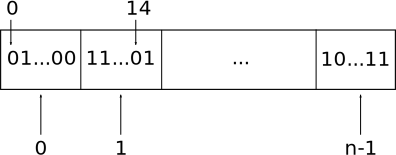
\includegraphics[width=0.40\textwidth]{figures/array_as_stream.pdf}
\caption{\label{fig:bitstream-indices} Array indices and bit indices in a bit stream}
\end{center}
\end{figure}

\item 
The C~programming language neither provides a type \emph{bit}
nor does it support random access to the bits of a bit stream.
In order to access the $i$-th bit of a bit sequence one typically
has to first access the byte with index $j = i/8$ and then access the 
bit $k = i \pmod{8}$ within this byte.
Note that in Figure~\ref{fig:bitstream-indices} 
bytes and bits are indexed in increasing order from the \emph{left}.
On the byte level, however, bits are often indexed from the \emph{right}.
For example, to access the $k$-th bit of a byte \inl{a} one can
shift this bit to the right by $7-k$ and extracts then the now
rightmost bit by performing a bit-wise \emph{and} with the value~1
%
\begin{verbatim}
   (a >> (7-k)) & 1
\end{verbatim}

\item
A \emph{bit sequence} is a consecutive sequence of bits within a bit stream
as represented in Figure~\ref{fig:bitsequence}.
\begin{figure}[hbt]
\begin{center}
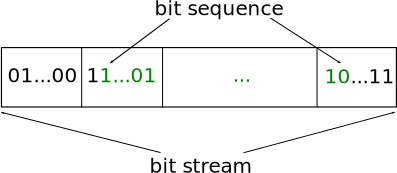
\includegraphics[width=0.40\textwidth]{figures/bit_sequence.pdf}
\caption{\label{fig:bitsequence} A bit sequence within a bit stream}
\end{center}
\end{figure}

A bit sequence is given by the position of its first bit (a bit index in the bit stream)
and its \emph{length}, that is, the number of bits it contains.

\item

A bit sequence that starts at bit index $p$ and that consists of
length $l \geq 0$ is refered to \emph{valid} (with respect to a bit stream of length $n$)
if the following conditions are satisfied
\begin{align*}
  0 &\leq p < 8n \\
  0 &\leq p + l \leq 8n
\end{align*}

Not that only the bits with indices $p \leq i < p + l$ are to be accessed
but not the bit with index~$p+l$.

\end{itemize}

We assume that the C-types \inl{unsigned int} and \inl{int}, which
are used in the implementation to represent indices, counting and error codes,
have a width of~32~bits.
We point this out here because we conducted the verification on a platform with
these characteristics.

As an aside, MISRA-C discourages the use of ``generic'' integer types
such as \inl{int} and \inl{unsigned int} and recommends the use of integer types whose names
contain the exact width.


\chapter{The \bitwalker functions in more detail}

\section{The public interface of \bitwalker}
\label{sec:bitwalker-public}

This section describes the public interface of \bitwalker.

\subsection{The structure \bitwalkertype}


The type \bitwalkertype is defined as follows\\[1em]

\begin{lstlisting}[style=acsl-block]
   struct  T_Bitwalker_Incremental_Locals
   {
       uint8_t       *Bitstream;
       unsigned int  Length;
       unsigned int  CurrentBitposition;
   };
\end{lstlisting}


\paragraph{Description}~

\begin{itemize}

   \item \inl{Bitstream} is  the start address of a valid bit stream.
   \item \inl{Length} is the length of the bit stream, that starts at \inl{Bitstream}.
   \item \inl{CurrentBitposition} is a valid bit index in
              the bit stream given by \inl{Bitstream} and \inl{Length}

\end{itemize}

\paragraph*{Remark}
The field \inl{Length} will be passed to \peek and \poke as \inl{BitstreamSize}.
This might be confusing because those functions also have an argument 
named~\inl{Length}.

\clearpage

\subsection{Informal Specification of \inl{Bitwalker_IncrementalWalker_Init}}

In this section we specify the function \init.
 The function  initializes object of the type \bitwalkertype.
The function signature reads:\\[1em]


\begin{lstlisting}[style=acsl-block]
void Bitwalker_IncrementalWalker_Init(
        T_Bitwalker_Incremental_Locals *Locals,
        uint8_t Bitstream[],
        unsigned int Size,
        unsigned int FirstBitposition);
\end{lstlisting}


\paragraph{Preconditions}
\begin{itemize}
   \item  \inl{Locals} is a dereferenceable pointer.
   \item \inl{Bitstream} is  the start address of a valid bit stream.
   \item \inl{Size} is the length of the bit stream, that starts at \inl{Bitstream}.
   \item \inl{FirstBitposition} is a valid bit index in the bit stream given by \inl{Bitstream} and \inl{Size}
\end{itemize}

\paragraph{Description}~

The function \init assigns
\begin{itemize}
    \item \inl{Bitstream}  to \inl{Locals->Bitstream}.
    \item \inl{Size} to \inl{Locals->Length}
    \item \inl{FirstBitposition} to \inl{Locals->CurrentBitposition}
\end{itemize}

\clearpage

\subsection{Informal Specification of \inl{Bitwalker_IncrementalWalker_Peek_Next}}

The function \peeknext reads a sequence from a bit stream 
and increments the current position in the bit stream by the 
length of the read bit sequence.
Its function signature reads as follows:\\[1em]


\begin{lstlisting}[style=acsl-block]
uint64_t Bitwalker_IncrementalWalker_Peek_Next(
    T_Bitwalker_Incremental_Locals *Locals,
    unsigned int Length);
\end{lstlisting}


\paragraph{Preconditions}
\begin{itemize}
  \item  \inl{Locals} must be dereferenceable
  \item \inl{Length} is the length of the bit sequence and shall be less or equal~64
  \item \inl{Locals->CurrentBitposition} $\leq$ \inl{UINT_MAX} $-$ \inl{Length}
\end{itemize}

\paragraph{Description}~

\peeknext reads a bit sequence from a bit stream and returns it as~64 bit integer.

\fxfatal{describe more precisely, see \peek}

If the bit sequence is not valid the function shall return \inl{0}.

The function increments the value \inl{Locals->CurrentBitposition} by \inl{Length}.

\fxfatal{does it make sense to increment in the case of an invalid bit sequence?}

\clearpage

\subsection{Informal Specification of \inl{Bitwalker_IncrementalWalker_Peek_Finish}}


 The function signature reads:\\[1em]

\begin{lstlisting}[style=acsl-block]
int Bitwalker_IncrementalWalker_Peek_Finish(
        T_Bitwalker_Incremental_Locals *Locals);
\end{lstlisting}

\paragraph{Preconditions}
\begin{itemize}
   \item  \inl{Locals} must be dereferenceable
\end{itemize}

\paragraph{Description}~

The function  returns \inl{Locals->CurrentBitposition}.
It does not change any variables.

\paragraph*{Remark} The return value of this function is \inl{int} despite
the fact that it returns a value of type \inl{unsigned int}.
This does not make much sense and should best be avoided.

\clearpage

\subsection{Informal Specification of \inl{Bitwalker_IncrementalWalker_Poke_Next}}

The function \pokenext writes a bit sequence into a bit stream 
and increments the current position in the bit stream by the 
length of the read bit sequence.\\[1em]


\begin{lstlisting}[style=acsl-block]
int Bitwalker_IncrementalWalker_Poke_Next(
        T_Bitwalker_Incremental_Locals *Locals,
        unsigned int Length,
        uint64_t Value);
\end{lstlisting}


\paragraph{Preconditions}
\begin{itemize}
    \item  \inl{Locals} must be dereferenceable
    \item \inl{Locals->CurrentBitposition} + \inl{Length} is less than or equal \inl{UINT_MAX}
\end{itemize}

\paragraph{Description}~

We specify \pokenext as follows:
The function \poke converts a 64-bit unsigned integer to a bit sequence and 
writes it into a bit stream.

For $0 \leq x$ exists a shortest sequence of~0 and~1
$(b_0, b_1,\ldots,b_{n - 1})$
such that
\begin{align}
    \sum_{i=0}^{n-1} b_i \cdot 2^{(n - 1) - i} = x.
\end{align}

The function \pokenext tries to store the sequence $(b_0, b_1,\ldots,b_{n - 1})$
in the bit sequence of \inl{Length} bits that starts
at bit index \inl{Locals->CurrentBitposition}.

The return value depends on  the following cases:
\begin{itemize}
    \item  If the bit sequence is not valid \peeknext  returns $-1$.
    \item  If the bit sequence is valid, then there are two cases:
\begin{itemize}
\item
If $x$ is greater or equal than $2^\mathtt{Length}$, then~$x$
cannot be represented as bit sequence $(b_0, b_1,\ldots,b_{\mathtt{Length} - 1})$.
\pokenext returns then~$-2$.

\item
If $x$ is less the $2^{\mathtt{Length}}$, then  the sequence
$(\overbrace{0,\ldots,0}^{\mathtt{Length}-n},b_0, b_1,\ldots,b_{n - 1})$
is stored in the bit stream starting at \inl{Locals->CurrentBitposition}.
The return value of the function \pokenext is 0.

\end{itemize}
\end{itemize}

Regardless of whether the poke was successful \pokenext sets the value  \inl{Locals->CurrentBitposition} to the first position behind the sequence that it tired to poke.
 All other components of the record \inl{Locals} remain unaltered.


\fxfatal{does it make sense to increment in the case of an invalid bit sequence?}

\clearpage

\subsection{Informal Specification of \inl{Bitwalker_IncrementalWalker_Poke_Finish}}

 The function signature reads:\\[1em]

\begin{lstlisting}[style=acsl-block]
int Bitwalker_IncrementalWalker_Poke_Finish(
        T_Bitwalker_Incremental_Locals *Locals);
\end{lstlisting}

\paragraph{Preconditions}
\begin{itemize}
    \item  \inl{Locals} must be dereferenceable
\end{itemize}

\paragraph{Description}~

The function  returns \inl{Locals->CurrentBitposition}.

\paragraph{Remark*}
The functions \peekfinish and\\
\pokefinish have the same specification.
Moreover, both function return an object of type \inl{unsigned int} as \inl{int}
for which no convincing reason is available.







\section{Specification of \peek and \poke}
\label{sec:bitwalker-private}

This section describes the functions \peek and \poke that 
are used for the implementation of some functions in Section~\ref{sec:bitwalker-public}.

\subsection{Informal specification of \peek}
\label{sec:informal-peek}

Now we specify \peek with the introduced auxiliary concepts.
The function \peek reads a bit sequence from a bit stream
and converts it to an integer.

Its function signature reads as follows:

\begin{lstlisting}[style=acsl-block]
uint64_t  Bitwalker_Peek(unsigned int Startposition, 
                         unsigned int Length,
                         uint8_t Bitstream[],
                         unsigned int BitstreamSizeInBytes);
\end{lstlisting}


\paragraph{Arguments and Preconditions}~

The arguments of \peek have the following purpose:
\begin{itemize}
    \item \inl{Startposition} is the bit index in the bit stream 
    where the bit sequence starts.
    \item \inl{Length} is the length of the bit sequence.
    \item \inl{Bitstream} is the array which provides the bit stream.
    \item \inl{BitstreamSizeInBytes} is the length of the array 
    containing the bit stream. 
\end{itemize}

The following preconditions shall hold for the function arguments.
Note that additional constraints are implicitly expressed by the use
of \emph{unsigned} integer types.

\begin{itemize}
\item \inl{Bitstream} is a valid array of length \inl{BitstreamSizeInBytes}

\item \inl{Length} $\leq$ \inl{64} and

\item \inl{Startposition} $\leq$ \inl{UINT_MAX} - \inl{Length}.
      This condition expresses that no arithmetic overflows shall occur
      when evaluating \inl{Startposition + Length}.
\end{itemize}

\paragraph{Description}~

As mentioned, the function \peek reads a bit sequence from a bit stream
and converts it to a 64-bit unsigned integer.

For a bit sequence $(b_0, b_1,\ldots,b_{n - 1})$ the function \peek returns the sum
\begin{align}
\label{eq:peek-result}
    \sum_{i=0}^{n-1} b_i \cdot 2^{(n - 1) - i} 
\end{align}

Note that is a higher-level description than what is done in the source code.
There is, in our opinion, not much point to reflect all of the low-level bit operations
into the specification if a clearer description is at hand.

If the bit sequence is not valid, then \peek shall return~0.
We were wondering why the implementation maps an illegal input to a legitimate output.
The code providers argued along the lines that this error condition was not
considered important enough to be properly reported.
One can interpret this design decision as an attempt to increase the
robustness of the function against illegal values.
In general, we recommend to explicitly describe all error conditions
and to devise a consistent error detection and error recovery strategy.


\subsection{Informal specification of \poke}
\label{sec:informal-poke}

In this section we examine the function \poke
in the same manner as we did it for \peek.

The function \poke converts an integer to a bit sequence and writes it
into a bit stream.
Its function signature reads as follows:
\begin{lstlisting}[style = acsl-block]
int      Bitwalker_Poke(unsigned int Startposition,
                        unsigned int Length,
                        uint8_t Bitstream[],
                        unsigned int BitstreamSizeInBytes,
                        uint64_t Value);
\end{lstlisting}


\paragraph{Arguments and Preconditions}~

The arguments have the following purpose:

\begin{itemize}
    \item \inl{Startposition} is the bit index in the bit stream 
    where the bit sequence starts.
    \item \inl{Length} is the length of the bit sequence.
    \item \inl{Bitstream} is the array which provides the bit stream.
    \item \inl{BitstreamSizeInBytes} is the length of the array 
    containing the bit stream. 
    \item \inl{Value} is the integer which shall be converted into a bit sequence.
\end{itemize}

The following conditions shall hold for the function arguments:

\begin{itemize}
\item \inl{Bitstream} is a valid array of length \inl{BitstreamSizeInBytes}

\item \inl{Startposition + Length} is less than \verb"UINT_MAX".
\end{itemize}

Note that additional constraints are implicitly expressed by the use
of \emph{unsigned} integer types.


\paragraph{Description}~

Now we can specify \poke as follows:
The function \poke converts a 64-bit unsigned integer to a bit sequence and 
writes it into a bit stream.

For $0 \leq x$ exists a shortest sequence of~0 and~1
$(b_0, b_1,\ldots,b_{n - 1})$
such that
\begin{align}
    \sum_{i=0}^{n-1} b_i \cdot 2^{(n - 1) - i} = x.
\end{align}

The function \poke tries to store the sequence $(b_0, b_1,\ldots,b_{n - 1})$
in the bit sequence of \inl{Length} bits that starts
at bit index \inl{Startposition}.

The return value of \poke depends on the following three cases:

\begin{itemize}
\item 
If the bit sequence is not valid, then \poke returns~$-1$.

\item 
If the bit sequence is valid, then there are two cases:

\begin{itemize}
\item
If $x$ is greater or equal than $2^\mathtt{Length}$, then~$x$
cannot be represented as bit sequence $(b_0, b_1,\ldots,b_{\mathtt{Length} - 1})$.
\poke returns then~$-2$.

\item
If $x$ is less the $2^{\mathtt{Length}}$, then  the sequence
$(\overbrace{0,\ldots,0}^{\mathtt{Length}-n},b_0, b_1,\ldots,b_{n - 1})$
is stored in the bit stream starting at \inl{Startposition}.
The return value of \poke is 0.

\end{itemize}
\end{itemize}



\end{document}
